\documentclass[12pt]{article}
\usepackage{amsmath}
\usepackage[english]{babel}
\usepackage{caption}
\usepackage{float}
\usepackage{graphicx}
\usepackage[utf8]{inputenc}
\usepackage{subcaption}
\usepackage{epsfig}

\title{Homework 3: Practicing with \LaTeX\ }
\author{Mohammad Khan}
\date{\today}

\begin{document}

\maketitle

\section{Working with Bullets}

\subsection{Plain Bullets}

Here is a list of what I enjoyed about class this semester.
\begin{itemize}
\item Throughout the semester, it was easy for me to access the lab because it was opened all the time.
\item Some tutorials and homeworks had a great amount of mathematical content, and they helped me in learning how we can do calculations in IDL. 
\item The introduction of Latex and Python in an IDL course is very helpful because these softwares are used in various fields.
\end{itemize}

\subsection{Numbering}
Here is a list of what I disliked about class this semester.
\begin{enumerate}
\item The book does not contain good examples of procedures and functions despite the fact that we used long "for loops" and "while loops" in our assignments. The examples in the book are very basic.
\item Sometimes the due dates to submit assignments were very close, and it was stressful to get them done by their due dates.
\item I still feel like I did not learn all of the IDL content covered in this class. 
\end{enumerate}

\section{Working with Equations}

\subsection{The Euler-Lagrange Equation}
This is the Euler-Lagrange equation:

\[
\sum_{j=0}^n (-1)^j \partial_{ \mu_{1}\ldots\mu_{j} }^j\left(\frac{
\partial \mathcal{L} }{\partial f_{i, \mu_1 \dots \mu_{j} } }\right
 ) = 0
\]
where $\mu_{1}\ldots \mu_{j}$ implies the sum over indices that span the
number of variables.

\section{Working with Tables}

\begin{table}[h!]
 \centering
 \begin{tabular}{ c | c | c }
 \hline
 Favorite Foods & Favorite Bands & Favorite IDL Commands \\ \hline
 Indian Curry & Metallica & transpose \\
 Pizza & The Ramones & findgen \\
 Burger & Guns N' Roses & cp \\ \hline
\end{tabular}
 \caption{I like several other items from each category, but those are my favorites.}
\end{table}

\section{Working with a Figure}
Here is an image. 
\begin{figure}[H]
 \centering
 \includegraphics[width=0.5\textwidth]{plot.ps}
 \caption{Scatter plot of the data. I liked the fact that how this tutorial generated a nice scatter plot, and I disliked that it was hard to fit the line of best fit}
\end{figure}

\section{Working with Multiple Figures}

\begin{figure}[H]
 \centering

 \begin{subfigure}[h!]{0.5\textwidth}
 \includegraphics[width=\textwidth]{/home/mkhan/Desktop/milkyway.jpg}
 \caption{Beautiful picture of our Milky Way Galaxy}
 \end{subfigure}
 ~
 \begin{subfigure}[h!]{0.5\textwidth}
 \includegraphics[width=\textwidth]{/home/mkhan/Desktop/whirlpoolgalaxy.jpg}
 \caption{Picture of whirlpool galaxy}
 \end{subfigure}
 \caption{Two good looking galaxies}

\end{figure}
\end{document}
